\section{Introduction}\label{intro}
In Astronomy, instruments with higher angular resolution allows us to measure ever smaller structures in the sky. For Radio frequencies, the angular resolution is bound to the antenna dish diameter, which puts practical and financial limitations on the highest possible angular resolution. Radio Interferometers get around this limitation by using several smaller antennas instead. Together, they act as a single large antenna with higher angular resolution at lower financial costs compared to single dish instruments.

Retrieving the observed image for Radio Interferometer becomes difficult. The Interferometer does not measure pixels of the sky. Instead, it measures an incomplete set of Fourier components. To retrieve the image, we have to solve the the Radio Interferometric Inverse Problem. We try to find the observed image, while we only know an incomplete set of Fourier Components. Due to the incomplete measurements, the inverse Problem is ill-posed, meaning we have a large number of possible images that fit the measurements. To solve this, image reconstruction algorithms try to find the most likely observed image.

Image reconstruction algorithm which tackle the ill-posed inverse problem. We have two dimensions, reconstructing an image which is as close as possible to the truly observed one, and finding an image as fast as possible.

New Radio Interferometers produce an ever larger number of Fourier Components. Calculating an image in a reasonable timeframe becomes an issue. Distribution Necessary. But the Radio Interferometric Inverse Problem so far has been difficult to distribute.


\subsection{Radio Interferometric Inverse Problem}
An example of the Inverse Problem is shown in figure \ref{intro:inversefig}. The image \ref{intro:inversefig:reconstruction} shows a reconstruction The image \ref{intro:inversefig:uvspace} shows the measurements of the MeerKAT Radio Interferometer in the Fourier space. Each dot represents a sampled Fourier component. Each antenna pair creates a sample. Each pair is called a baseline. 

What points are sampled are defined by the Antenna layout. Sampling pattern is non-uniform in the Fourier space. Meaning we have more densely sampled areas and more sparsely sampled areas. The image \ref{intro:inversefig:uvspace} clearly shows the incompleteness of the measurements. We have "holes" in the uv-space, which is missing information.

What is an Observation. Over a time window. Create an image over several hours of measurements. This increases the number of samples that we have to deal

Noise in the Fourier Components. Amplitude and phase noise. 


\begin{figure}[htp]
	% preliminary
	\sbox\twosubbox{%
		\resizebox{\dimexpr.9\textwidth-1em}{!}{%
			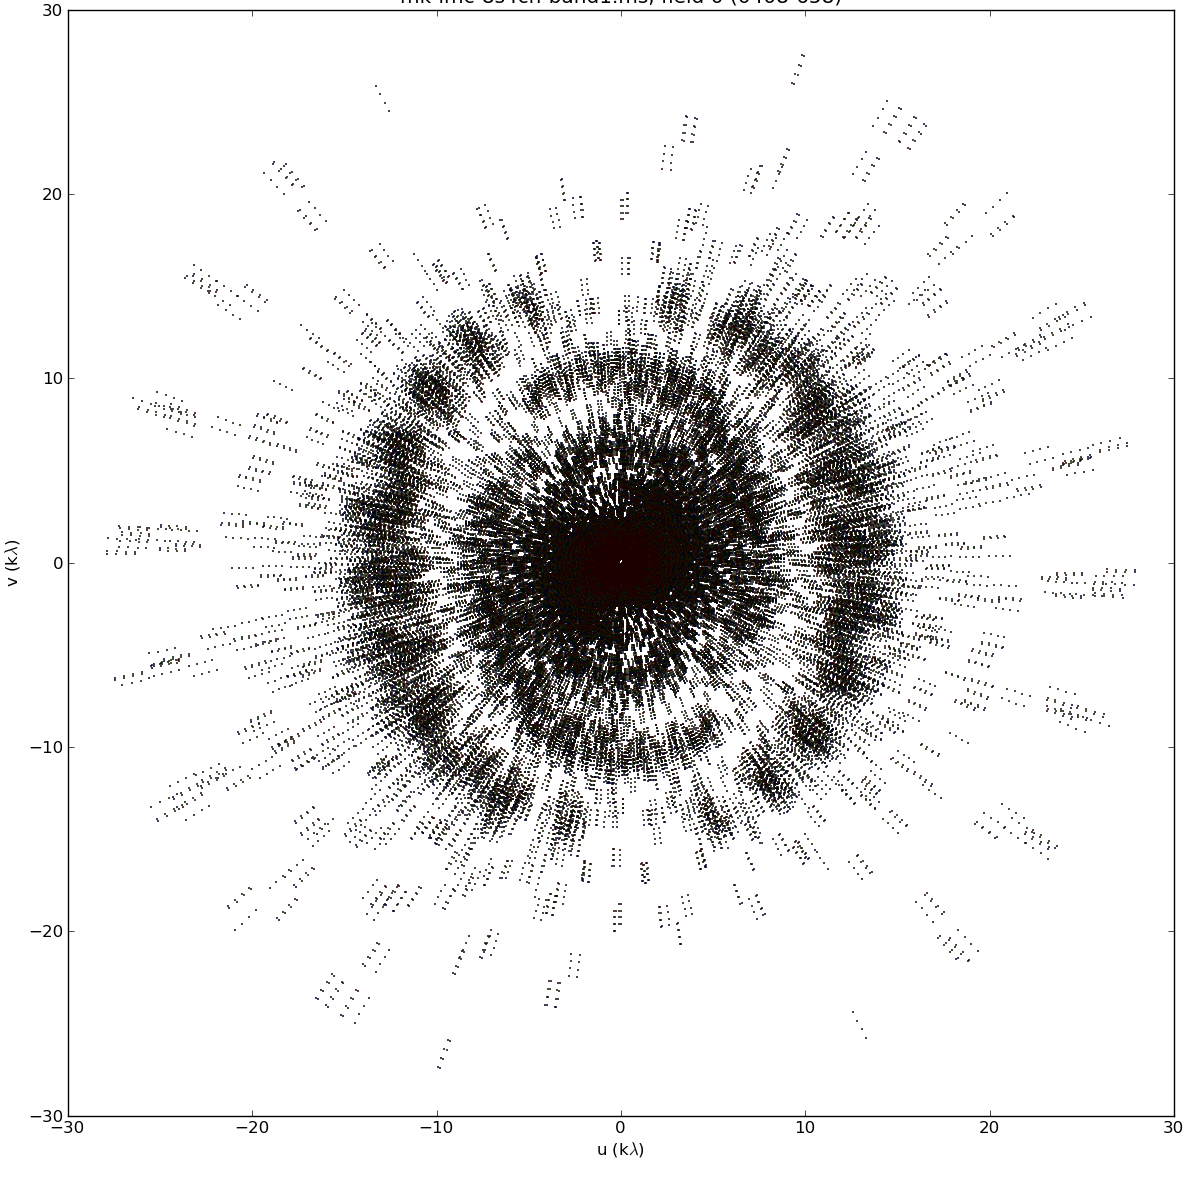
\includegraphics[height=3cm]{./chapters/01.intro/meerkat_uv2.png}%
			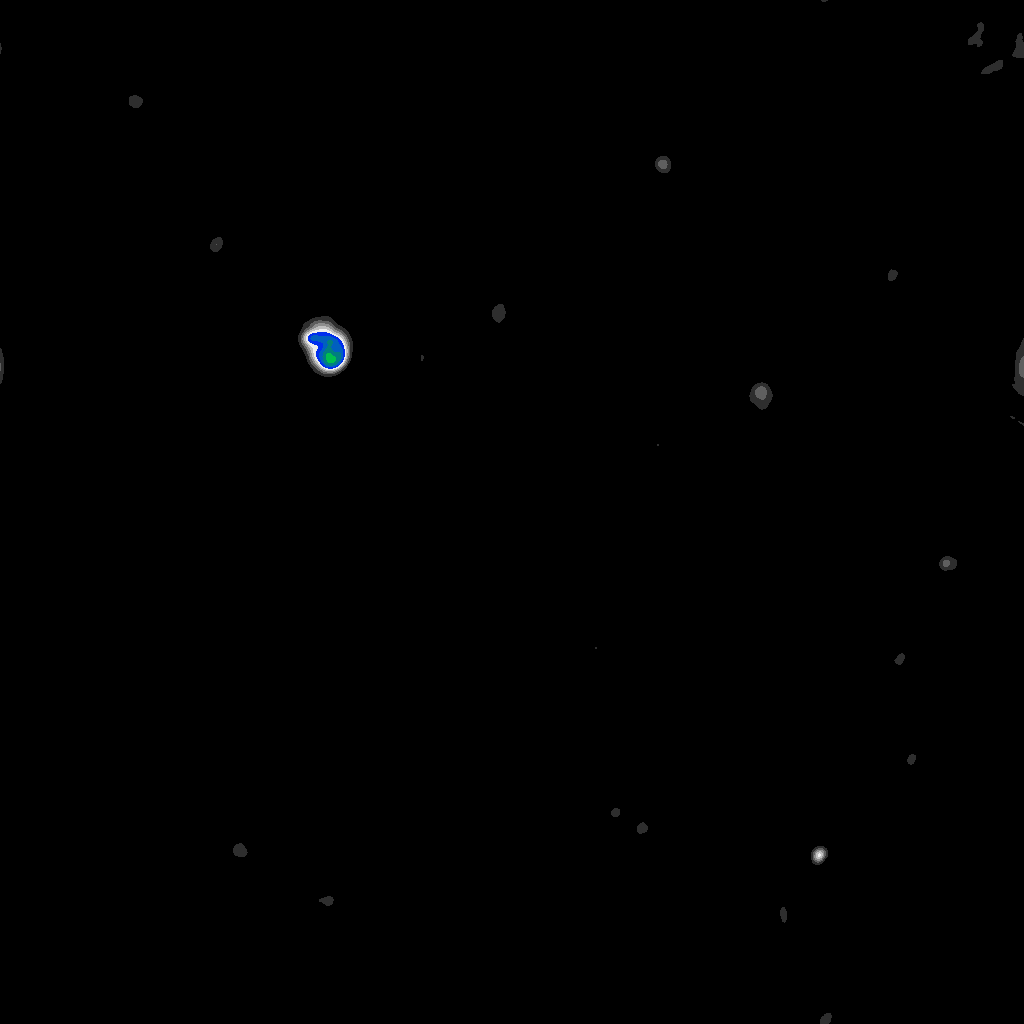
\includegraphics[height=3cm]{./chapters/01.intro/mk2/clean.png}%
		}%
	}
	\setlength{\twosubht}{\ht\twosubbox}
	
	% typeset
	\centering
	\subcaptionbox{Measurements of the MeerKAT Radio Interferometer.\label{intro:inversefig:uvspace}}{%
		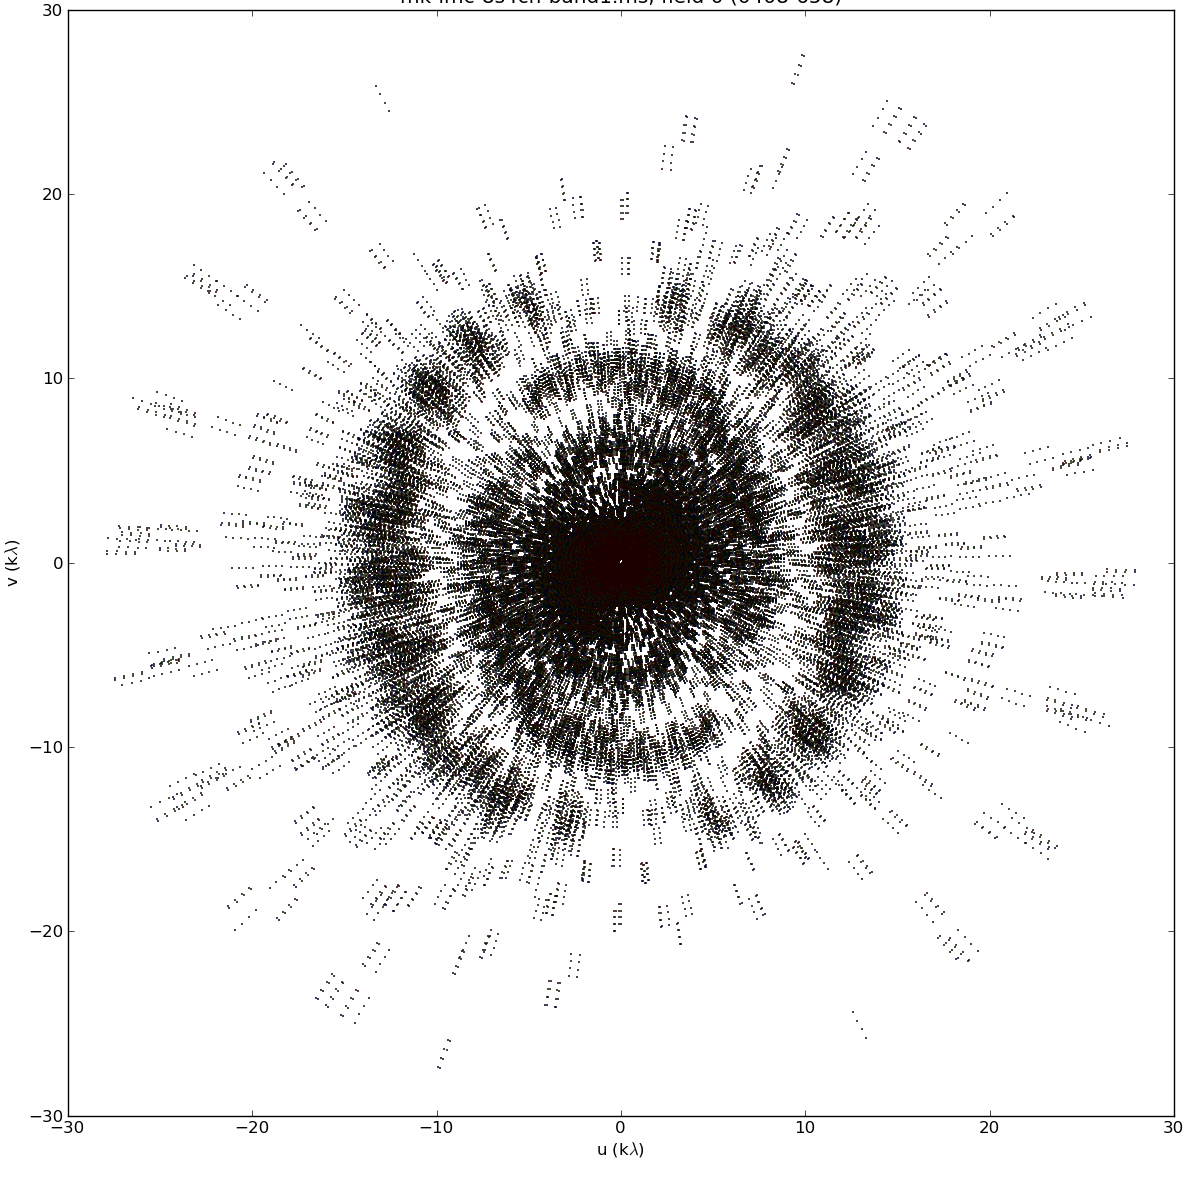
\includegraphics[height=\twosubht]{./chapters/01.intro/meerkat_uv2.png}%
	}\quad
	\subcaptionbox{A reconstruction which fits the observation.\label{intro:inversefig:reconstruction}}{%
		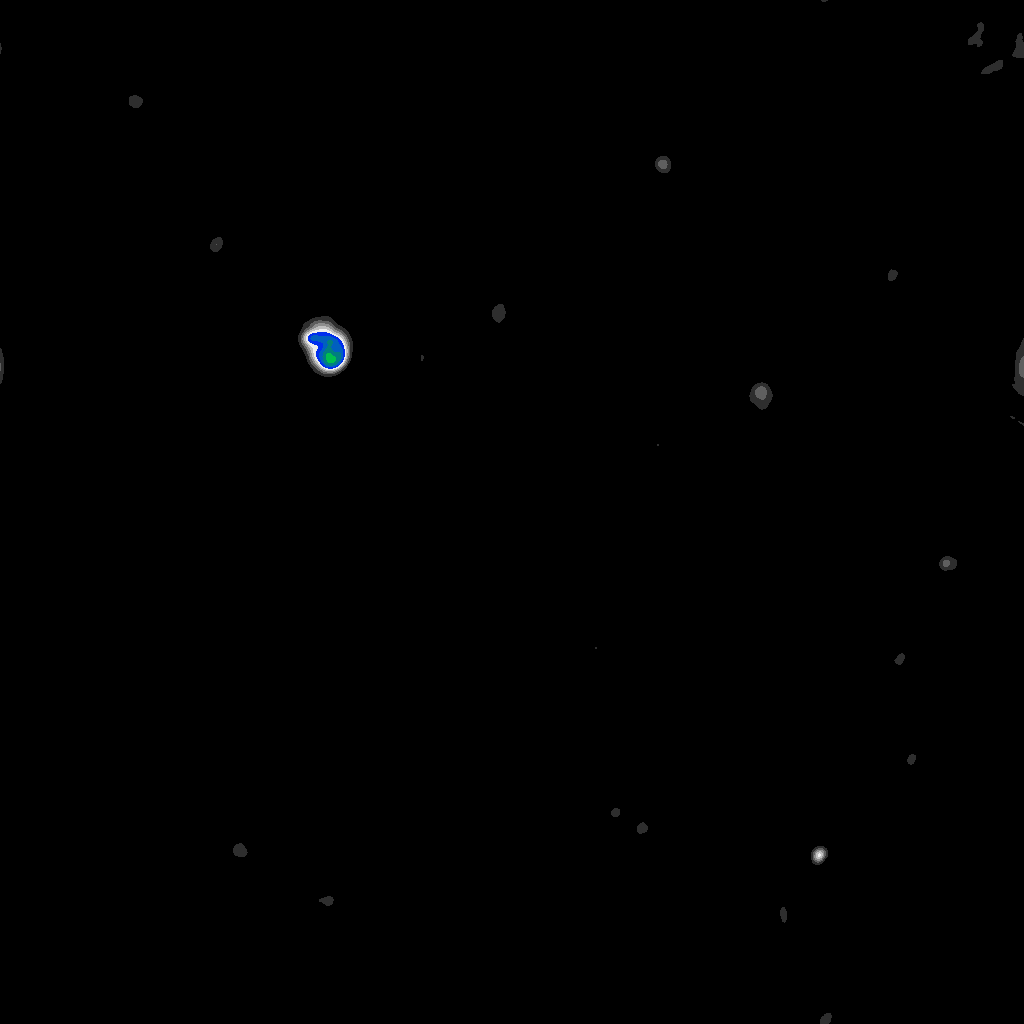
\includegraphics[height=\twosubht]{./chapters/01.intro/mk2/clean.png}%
	}
	\caption{The Image Reconstruction Problem}\label{intro:inversefig}
\end{figure}


Inverse Problem, We have measurements and want to find the image matching the measurements. Incomplete, there are potentially infinite number of images fitting 
the measurements. This forms an Ill-Posed inverse problem. 
Overdetermined problem, we have magnitudes more Visibilities than Pixels in the image. But noise and holes in the 

For Distribution, details become important
Not the 2d Fourier Relationship.
Specific to Radio Interferometers


Or more formally in equation \eqref{intro:inverseproblem}


\begin{equation}\label{intro:inverseproblem}
V(u, v, w) = \int\int \frac{I(x, y)}{\sqrt{1 - x^2 - y ^2}} e^{2 \pi i [ux+vy+ w(\sqrt{1 - x^2 - y ^2} - 1)]} \: dx \: dy
\end{equation}

3d Fourier Relationship.

w-projection makes this difficult.

Difficult to calculate efficiently. $w$-term, and the non-uniform sampling pattern keeps us from using the FFT.

To solve this efficiently, the question is how this can be represented in a way that we can re-use the 2d fourier transform.


\begin{figure}[h]
	\centering
	\begin{subfigure}[b]{0.3\linewidth}
		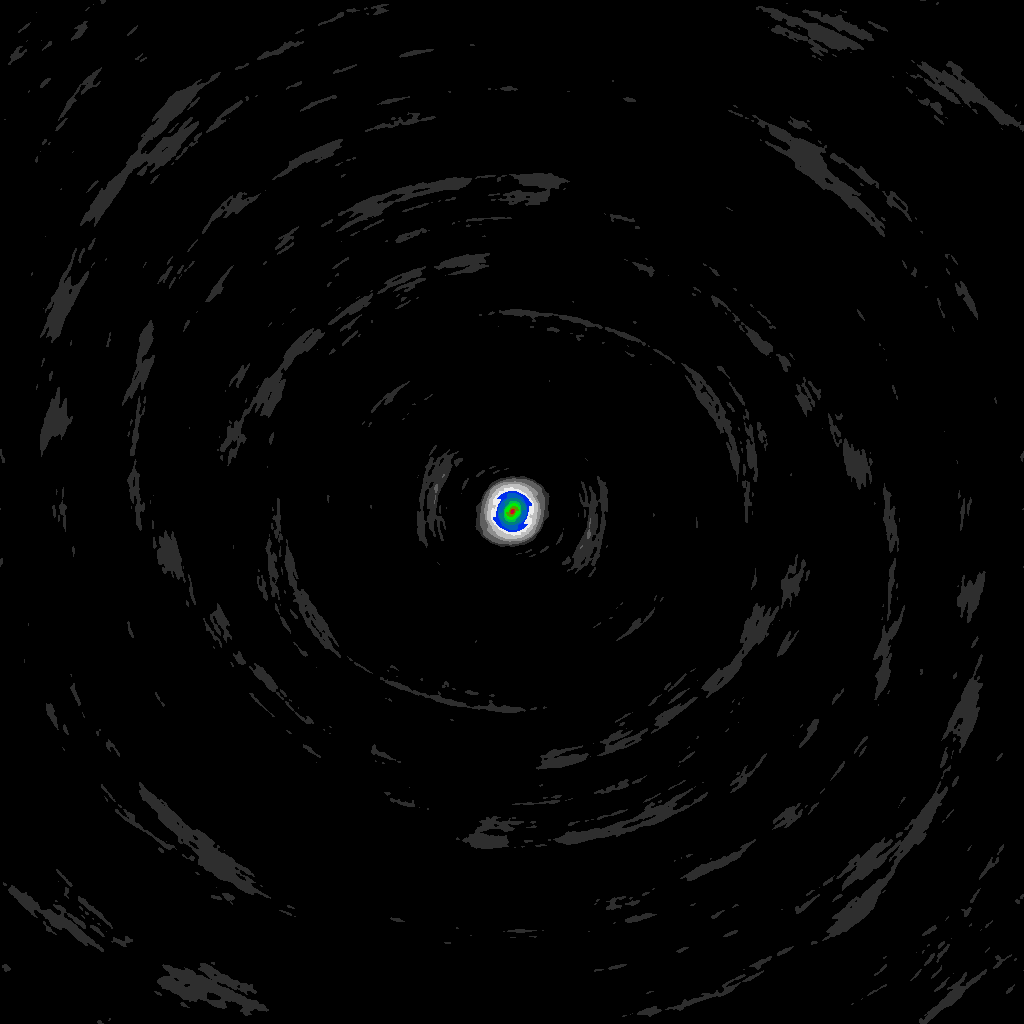
\includegraphics[width=\linewidth]{./chapters/01.intro/mk2/psf.png}
		\caption{CLEAN reconstruction \\with CASA standard parameters.}
		\label{results:points:tclean}
	\end{subfigure}
	\begin{subfigure}[b]{0.3\linewidth}
	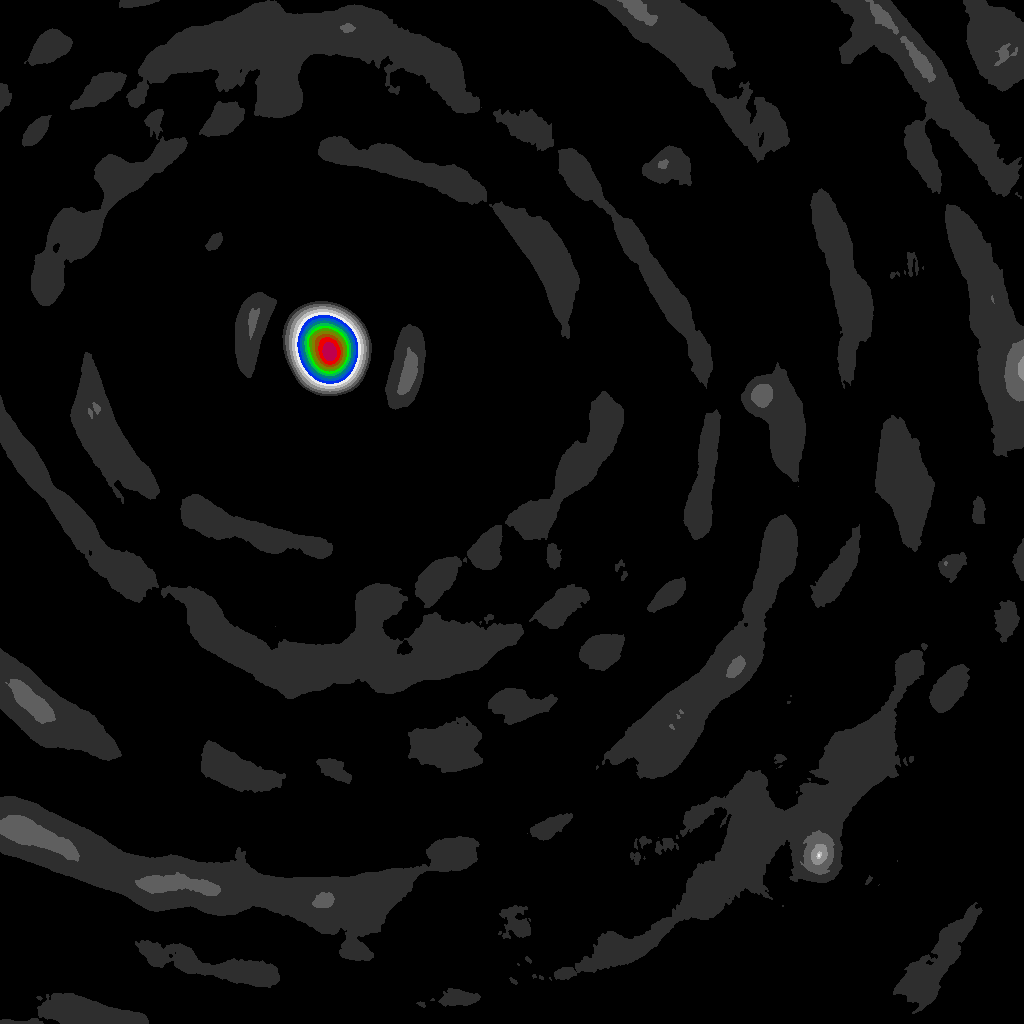
\includegraphics[width=\linewidth]{./chapters/01.intro/mk2/dirty.png}
	\caption{CLEAN reconstruction \\with CASA standard parameters.}
	\label{results:points:tclean}
	\end{subfigure}
	\begin{subfigure}[b]{0.3\linewidth}
		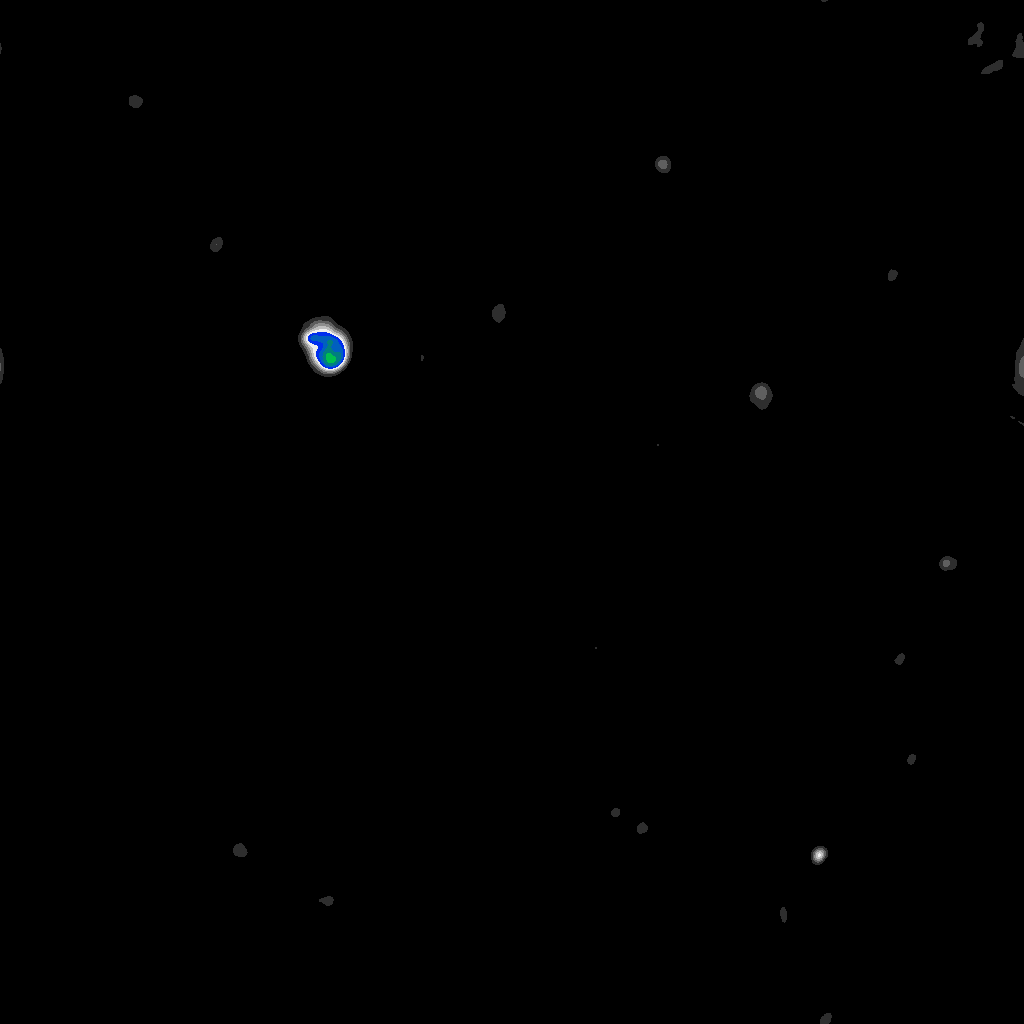
\includegraphics[width=\linewidth]{./chapters/01.intro/mk2/clean.png}
		\caption{CLEAN reconstruction \\with CASA standard parameters.}
		\label{results:points:tclean}
	\end{subfigure}

	
	\caption{Image reconstruction of two simulated point sources.}
	\label{results:points}
\end{figure}




\subsection{Radio Interferometric Image Reconstruction}

Solving the Ill-Posed inverse problem
Whole system.
From measurements to image reconstruction contains many different steps. In this project, we concern ourselves with the image reconstruction

\begin{figure}[h]
	\centering
	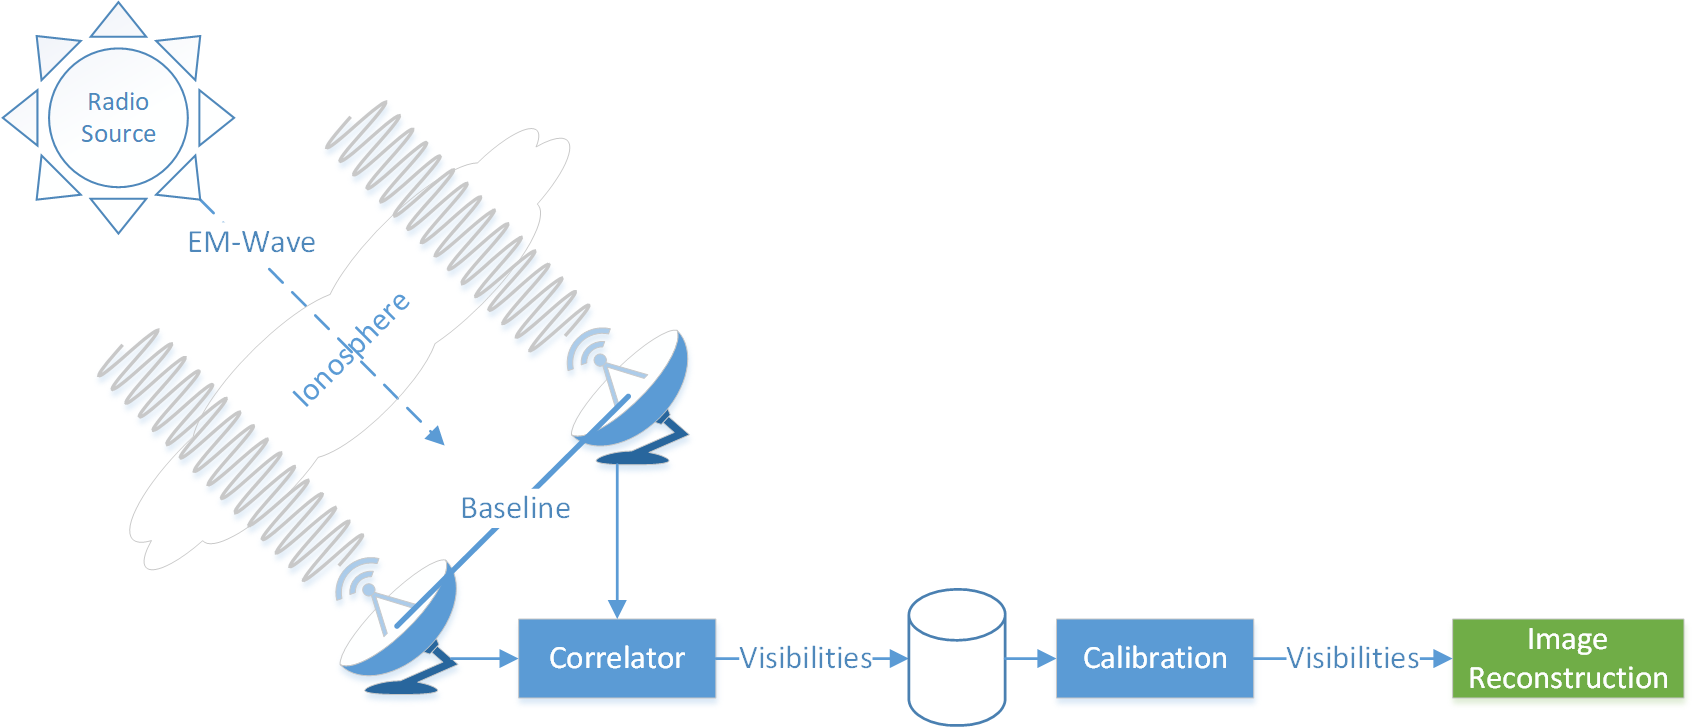
\includegraphics[width=0.80\linewidth]{./chapters/01.intro/system.png}
	\caption{Interferometer System}
	\label{intro:system}
\end{figure}

Calibration is not directly
Bad calibration can introduce a special error in the image.

Different ways of formulating the image reconstruction problem:
Interpolating the missing Visibilities
Deconvolution (also called "Minor Cycles")
Finding an image which fits the measurements

\subsubsection{The Major Cycle Architecture}
State of the art architecture used for reconstructing images. It Models the problem as deconvolution, and it needs three Operations:
\begin{itemize}
	\item Gridder
	\item FFT
	\item Deconvolution
\end{itemize}

The full algorithm is done 

\begin{figure}[h]
	\centering
	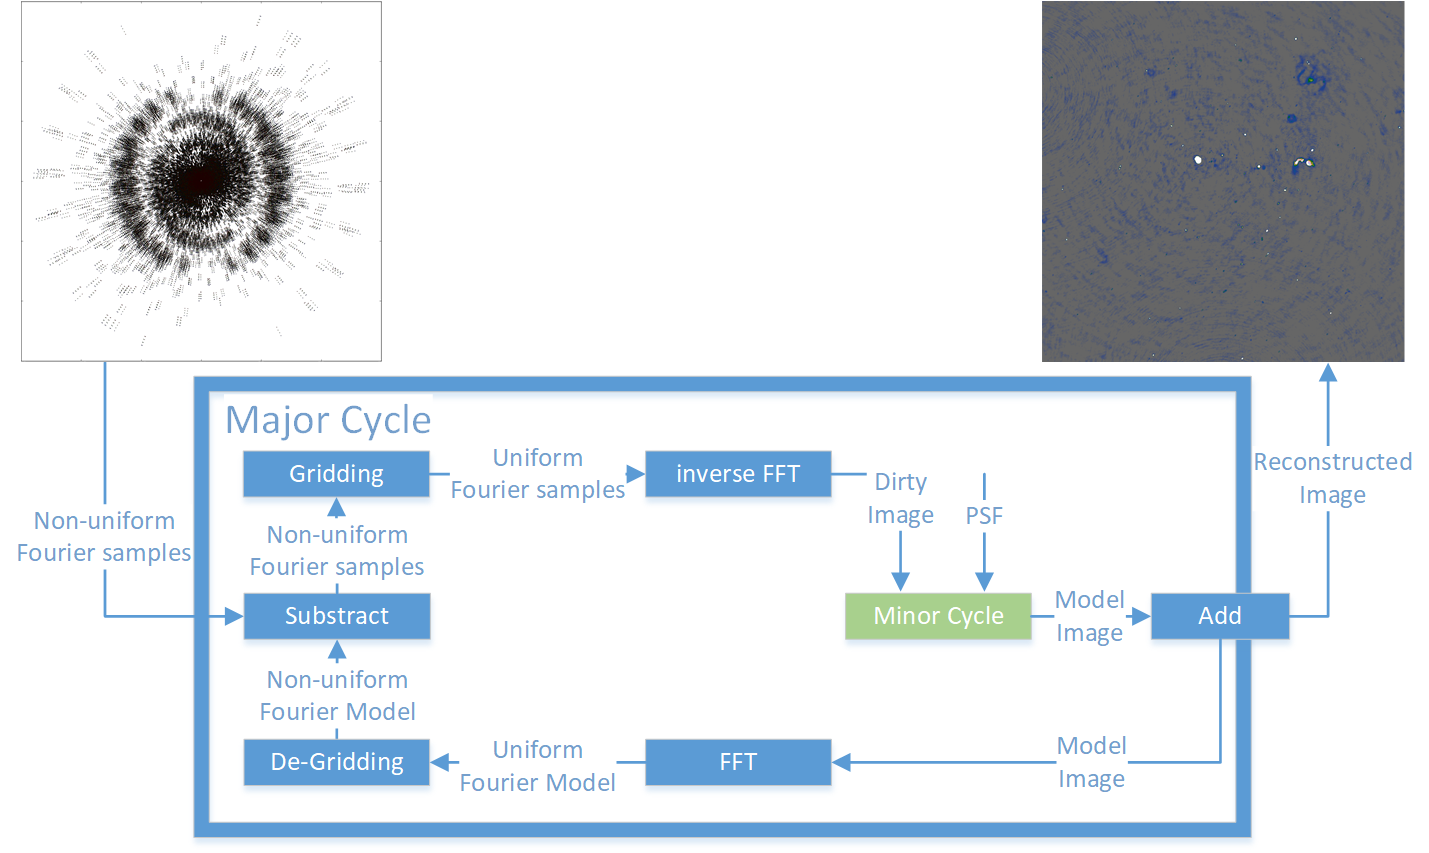
\includegraphics[width=0.80\linewidth]{./chapters/02.hypo/Major-Minor3.png}
	\caption{The Major Cycle Architecture}
	\label{intro:major}
\end{figure}

\subsubsection{ Deconvolution}
Other algorithms, mainly CLEAN
CLEAN




\subsection{Large scale Reconstruction Problem of MeerKAT}
New class of radio interferometers produce an ever increasing number of data.


Bottlenecks.
The Problem of Computation vs Quality
Image is magnitudes smaller than input data

Deconvolution with CLEAN.

Mostly Shared-Memory systems, large single machines.

GRIDDING Problem. The $w$-component of the Visibilities made this difficult. 

w-stacking, lately IDG. This has made the Gridding more efficient.

Use IDG to Distribute the Gridding.




CLEAN deconvolution still hard to parallelize.


\subsubsection{Gridding on the GPU}

\subsubsection{Theory of Compressed Sensing}











